% $Id$
%\documentclass[handout]{beamer}
\documentclass{beamer}
\usepackage[utf8]{inputenc}
\usepackage[T1]{fontenc}
\usepackage[english,swedish]{babel}
\usepackage{url}
\usepackage{graphicx}
\usepackage{color}
\usepackage{subfig}
\usepackage{csquotes}
\usepackage[natbib,style=alphabetic,maxbibnames=99]{biblatex}
\addbibresource{msbintro.bib}
\setbeamertemplate{bibliography item}[text]

\mode<presentation>{%
  \usetheme{Frankfurt}
  \setbeamercovered{transparent}
  \usecolortheme{seagull}
}
\setbeamertemplate{footline}{\insertframenumber}

\title[Intro MSB]{%
  Introduktion till\\
  MSB:s metodstöd
}
\author{Carina Bengtsson och Daniel Bosk\footnote{%
  Detta verk är tillgängliggjort under licensen Creative Commons 
  Erkännande-DelaLika 2.5 Sverige (CC BY-SA 2.5 SE).
	För att se en sammanfattning och kopia av licenstexten besök URL 
	\url{http://creativecommons.org/licenses/by-sa/2.5/se/}.
}}
\institute[MIUN ITM]{%
  %Department of Information and Communication Systems (ICS),\\
  %Mid Sweden University, Sundsvall.
	%
  Avdelningen för informations- och kommunikationssytem (IKS),\\
  Mittuniversitetet, Sundsvall.
}
\date{\today}

%\pgfdeclareimage[height=0.65cm]{university-logo}{MU_logotyp_int_CMYK.pdf}
%\logo{\pgfuseimage{university-logo}}

\AtBeginSection[]{%
	\begin{frame}<beamer>{Översikt}
		\tableofcontents[currentsection]
	\end{frame}
}

\begin{document}

\begin{frame}
  \titlepage{}
\end{frame}

\begin{frame}{Översikt}
	\tableofcontents
	% You might wish to add the option [pausesections]
\end{frame}


% Since this a solution template for a generic talk, very little can
% be said about how it should be structured. However, the talk length
% of between 15min and 45min and the theme suggest that you stick to
% the following rules:  

% - Exactly two or three sections (other than the summary).
% - At *most* three subsections per section.
% - Talk about 30s to 2min per frame. So there should be between about
%   15 and 30 frames, all told.


\section[Metodstöd]{MSB:s metodstöd}

\subsection{MSB}

\begin{frame}{MSB}
  \begin{itemize}
    \item Myndigheten för samhällsskydd och beredskap.
    \item \enquote{MSB utvecklar, tillsammans med andra, individens och 
        samhällets förmåga att förebygga, hantera och lära av olyckor och 
        kriser.}
  \end{itemize}
\end{frame}

%\begin{frame}{MSB:s organisation}
%  \begin{figure}
%    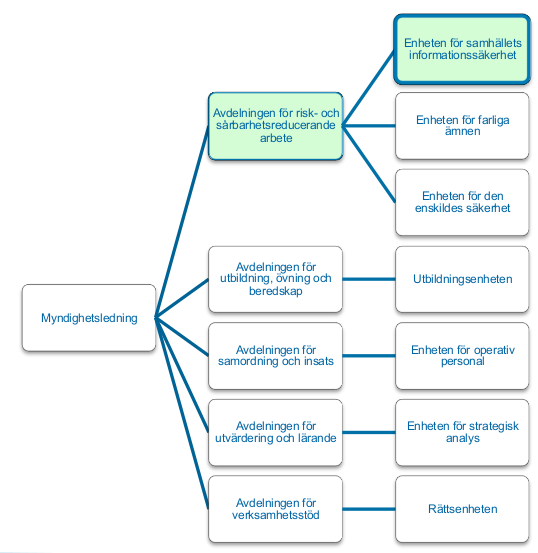
\includegraphics[height=0.7\textheight]{msb-organisation.png}
%    \caption{MSB:s organisation.}
%  \end{figure}
%\end{frame}

\begin{frame}{Varför behöver samhället detta?}
  \begin{itemize}
    \item Information är centralt i dagens samhälle.
    \item Tillgodoser behov för både individ och samhälle.
    \item Behöver undvika störningar av våra informationssystem.
  \end{itemize}
\end{frame}

\begin{frame}[allowframebreaks]{Tietohaveriet}
  \citet{Lindkvist2012tdf} ger följande sammanfattning:
  \begin{description}
    \item[Fredag e.m.] Tieto uppmärksammar en driftstörning.
      350 Apoteket-butiker tappar kontakt med sina IT-system.
      Många andra större organisationer drabbas också, bland andra ett större 
      logistikföretag.

    \item[Söndag e.m.] Tieto rapporterar maskinvarufel och påbörjar åtgärder.

    \item[Måndag f.m.] Logistikföretag kan inte sköta sin verksamhet och inte 
      nå sina anställda.
      Bilprovningen har totalstopp i IT-systemet -- dessa hanterar 20\,000 
      fordon om dagen -- resulterar i körförbud då Transportstyrelsen ej får in 
      godkända kontrollbesiktningar.
      Nacka kommun övergår till Facebook och Twitter för kommunikation.

    \item[Måndag e.m.] Socialkontoren i Nacka och Sollentuna kan ej betala ut 
      försörjningsstöd.
      Stockholm stads frånvarorapporteringssytem för skolorna ligger nere.

    \item[Onsdag lunch] Samtliga Apotek har fått tillbaka sina IT-system.

    \item[11 dagar] Logistikföretaget får tillbaka sitt IT-system.
      Verksamheten är fortfarande inte återställd två månader efter haveritet.

  \end{description}
\end{frame}

\subsection{Metodstödet}

\begin{frame}{Informationssäkerhet.se}
  \begin{itemize}
    \item MSB drev projektet SVISA\@: Stöd för Verksamheters 
      InformationsSäkerhetsArbete.

    \item Resulterade i \url{informationssäkerhet.se}.

    \item Ska ge praktiskt stöd för systematiskt informationssäkerhetsarbete.

  \end{itemize}
\end{frame}

\begin{frame}{Metodstödet}
  \begin{itemize}
    \item Stöd för att bedriva informationssäkerhetsarbete i en organisation.

    \item Förklarar hur man bygger ett ledningssystem för informationssäkerhet.

    \item Bör ses som ett \enquote{smörgåsbord}:
      \begin{itemize}
        \item Ta de delar som är aktuella för verksamheten.
        \item Tillämpa dem i den ordning som är lämpligt.
      \end{itemize}

    \item Informationssäkerhet är komplext:
      \begin{itemize}
        \item Krävs att den integreras i \emph{hela} organisationen: allt från 
          högsta ledningsnivå till lägsta operativa nivån.
      \end{itemize}

  \end{itemize}
\end{frame}

\begin{frame}{Metodstödet}
  \begin{figure}
    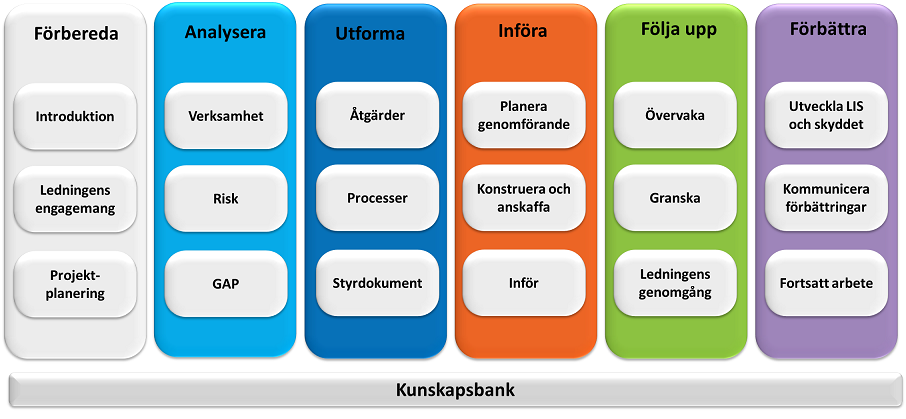
\includegraphics[width=\textwidth]{metodstod-overview.png}
    \caption{Översikt av metodstödet.}
  \end{figure}
\end{frame}


\section{Förbereda}

\subsection{Introduktion}

\begin{frame}{Vad är informationssäkerhet?}
  \begin{itemize}
    \item Uppstår tillsammans med andra processer och verksamheter.

    \item Informationssäkerheten i en verksamhet har inget egenvärde måste 
      integreras för att kunna skydda verksamheten.

  \end{itemize}
\end{frame}

\begin{frame}{Vad är informationssäkerhet?}
  \begin{itemize}
    \item Förmågan att bevara de krav och förväntningar som finns på 
      informationen i verksamheten.

    \item Bland annat att skydda från haverier likt Tieto---om det finns sådana 
      krav!

  \end{itemize}
\end{frame}

\begin{frame}{Krav och förväntningar på informationen}
  \begin{description}
    \item[Konfidentialitet] Informationen ska endast vara tillgänglig för 
      behörig.

    \item[Tillgänglighet] Informationen är användbar och finns till hands när 
      den behövs.

    \item[Riktighet] Informationen är exakt och fullständig.

  \end{description}
\end{frame}

\begin{frame}{Krav och förväntningar på informationen}
  \begin{description}
    \item[Spårbarhet] Vem har tagit del av eller förändrat information?
    \item[Oavvislighet] Det ska inte gå att förneka en handling.
    \item[Autentisering] Fastställa en entitets identitet.
    \item[Auktorisation] Att ge en autentiserad entitet vissa rättigheter.
  \end{description}
  Återkommer till dessa senare i kursen.
\end{frame}

\begin{frame}{Vad är informationssäkerhet?}
  \begin{figure}
    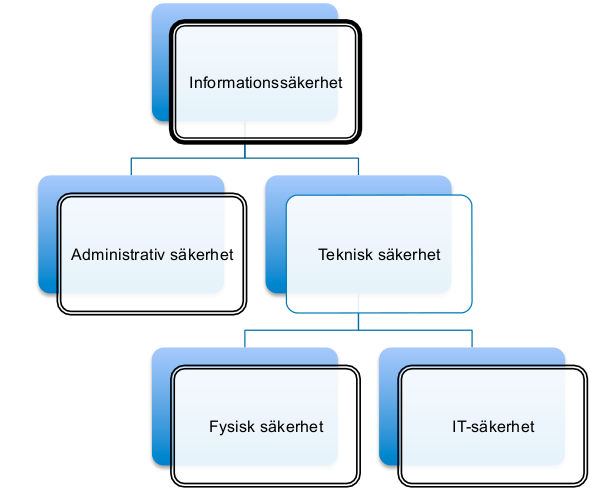
\includegraphics[height=0.7\textheight]{infosak-struktur.png}
    \caption{Informationssäkerhetens struktur.}
  \end{figure}
\end{frame}

\begin{frame}{Struktur}
  \begin{figure}
    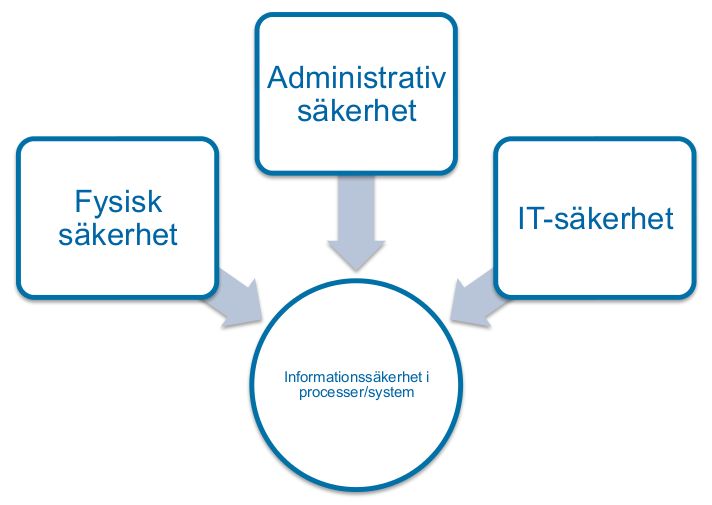
\includegraphics[height=0.7\textheight]{infosak-process.png}
    \caption{Att arbeta med informationssäkerhet.}
  \end{figure}
\end{frame}

\begin{frame}{Säkerheten är inte starkare än den svagaste länken}
  \begin{itemize}
    \item Svårgissat lösenord på post-it bredvid datorn.
    \item Oknäckbart kodlås på glasdörr.
    \item Det måste finnas förutsättningar för att arbeta säkert.
  \end{itemize}
\end{frame}

\begin{frame}{Varför skydda information?}{Frivilligt}
  Bra för verksamhetens
  \begin{description}
    \item[rykte:] vem låter ett företag hantera ens information om de är kända 
      för att göra det vårdslöst;

    \item[ekonomi:] gott rykte är bättre för ekonomin och kostnader för 
      säkerhetsincidenter minskar;

    \item[intern effektivitet:] inga förluster av information eller uppehåll 
      i arbetet, jämför med Tietohaveriet;

    \item[kvalitet:] följd blir att kvalietet på arbetet man utför ökar.

  \end{description}
\end{frame}

\begin{frame}{Varför skydda information?}{Obligatoriskt}
  \begin{description}
    \item[PUL 1998:204] säger att personuppgifter inte får hanteras och lämna 
      en verksamhet hur som helst;

    \item[Offentlighets- och sekretesslagen 2009:40] säger att viss information 
      \emph{ska} finnas tillgänglig för allmänheten medan annan information 
      \emph{inte} ska det.

    \item[Arkivlagen 1990:782] säger att myndigheter måste arkivera alla 
      allmänna handlingar.

    \item[MSBFS 2009:10] gäller myndigheters arbete med informationssäkerhet.

  \end{description}
\end{frame}

\begin{frame}{MSBFS 2009:10}
  \begin{itemize}
    \item På grund av ökat elektroniskt informationsutbyte i samhället ställs 
      nu krav på myndigheters informationssäkerhetsarbete.

    \item Författningen trädde i kraft 1 februari 2010.

  \end{itemize}
\end{frame}

\begin{frame}{MSBFS 2009:10}
  1 §   Denna författning innehåller bestämmelser om myndigheternas arbete med 
  informationssäkerhet och deras tillämpning av standarder i sådant arbete.
\end{frame}

\begin{frame}{MSBFS 2009:10}
  4 §   En myndighet ska i sitt arbete med att upprätthålla säkerhet i sin 
  informationshantering tillämpa ett ledningssystem för informationssäkerhet.
  Det innebär att myndigheten ska
  \begin{enumerate}
    \item upprätta en informationssäkerhetspolicy och andra styrande dokument 
      som behövs för myndighetens informationssäkerhet,
    \item utse en eller flera personer som leder och samordnar arbetet med 
      informationssäkerhet,
    \item klassificera sin information med utgångspunkt i krav på 
      konfidentialitet, riktighet och tillgänglighet,
    \item utifrån risk- och sårbarhetsanalyser och inträffade incidenter 
      avgöra hur risker ska hanteras, samt besl uta om åtgärder för 
      myndighetens informationssäkerhet,
    \item dokumentera granskningar och säkerh etsåtgärder av större betydelse 
      som har vidtagits.
  \end{enumerate}
\end{frame}

\begin{frame}{MSBFS 2009:10}
  5 §   Myndighetens ledning ska löpande informera sig om arbetet med 
  informationssäkerhet samt minst en gång per år följa upp och utvärdera 
  informationssäkerhetsarbetet på myndigheten.
\end{frame}

\begin{frame}{MSBFS 2009:10}
  6 §   En myndighets arbete enligt 4 och 5 §§ ska bedrivas i former enligt 
  följande etablerade svenska standarder för informationssäkerhet;
  \begin{itemize}
    \item Ledningssystem för informationssäkerhet -- Krav (SS-ISO/IEC 
      27001:2006 fastställd 2006-01-19), och
    \item Riktlinjer för styrning av informationssäkerhet (SS-ISO/IEC 
      27002:2005 fastställd 2005-08-12).
  \end{itemize}
\end{frame}

\begin{frame}{ISO 27000}
  \begin{itemize}
    \item Inte bara myndigheter som kan ha nytta av detta.

    \item Finns möjlighet för certifiering av ISO 27000 för alla 
      organisationer.

    \item MSB:s metodstöd är alltså anpassat efter dessa internationella 
      standarder.

  \end{itemize}
\end{frame}

\begin{frame}{Ledningssystem}
  \begin{itemize}
    \item Alla har ett \enquote{system} för att leda verksamheten.
  \end{itemize}
  \begin{quote}
    \blockcquote{lis}[.]{Ett formaliserat system som används för att göra 
      arbetet mer effektivt med avseende på uppställda mål.
    Det ska innehålla rutiner och ansvarsfördelningar i hur verksamheten leds 
    och bedrivs, finnas uppsatta mål och riktlinjer för hur de ska uppnås}
  \end{quote}
  \begin{itemize}
    \item Omfattar exempelvis organisationsstruktur, styrdokument, \dots
  \end{itemize}
\end{frame}

\begin{frame}{Ledningssystem för informationssäkerhet (LIS)}
  \begin{itemize}
    \item Bör integreras med övriga ledningssystemet!
    \item Syftar till att ordna informationssäkerhetsarbetet.
    \item Även hur man håller ordning: exempelvis arbetssätt, metoder.
    \item Styrdokument har en viktig roll i ett LIS\@.
  \end{itemize}
\end{frame}

\begin{frame}{Tillämpa LIS}
  Inte bara upprätta, utan även
  \begin{itemize}
    \item införa,
    \item driva,
    \item övervaka,
    \item granska,
    \item underhålla och förbättra
  \end{itemize}
  LIS inom ramen för verksamheten och riskerna.
\end{frame}

\begin{frame}{Styrdokument}
  \begin{itemize}
    \item Handlingsplaner, policyer, riktlinjer, \dots

    \item Policy: vad vill vi uppnå?
      En stor eller många små.

    \item I övrigt bör styrdokumenten integreras i verksamhetens nuvarande 
      struktur.

  \end{itemize}
\end{frame}

\begin{frame}{Informationssäkerhet på olika nivåer}
  \begin{figure}
    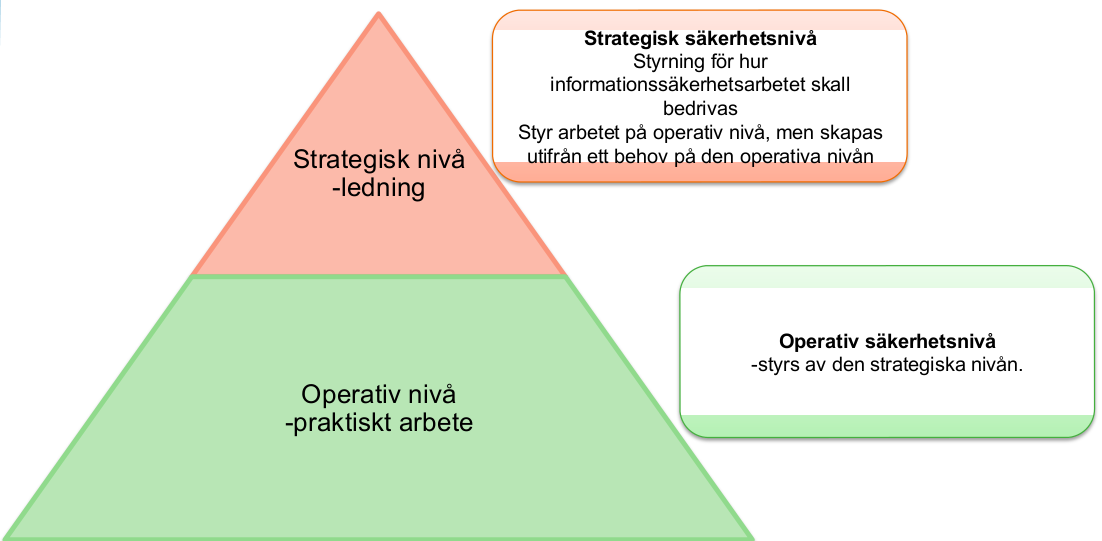
\includegraphics[width=\textwidth]{infosak-levels.png}
    \caption{De olika nivåerna där informationssäkerhetsarbete kan bedrivas.}
  \end{figure}
\end{frame}

\begin{frame}{Syftet med LIS}
  \begin{figure}
    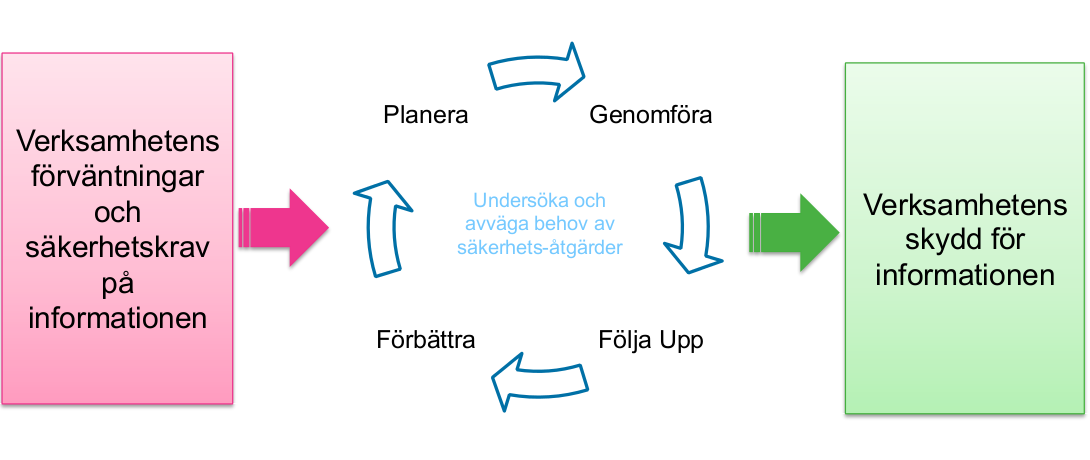
\includegraphics[width=\textwidth]{infosak-pdca.png}
    \caption{Att omvandla krav till aktivt skydd.}
  \end{figure}
\end{frame}

\begin{frame}{ISO 27001}
  \begin{itemize}
    \item Metodstödet beskriver hur man bygger upp ett LIS utifrån kraven i ISO 
      27001.

    \item ISO 27001 är en ständigt pågående systematisk process som strävar mot 
      ständiga förbättringar av arbetssätt och säkerhetslösningar 
      i informationssäkerhetsarbetet.

    \item Det är viktigt att anpassa detta efter den egna verksamheten -- men 
      det innebär inte att man kan hoppa över delar efter eget godtycke.

  \end{itemize}
\end{frame}

\begin{frame}{PDCA}
  \begin{description}
    \item[Plan] Förbereda, analysera, utforma.
    \item[Do] Införa.
    \item[Check] Följa upp.
    \item[Act] Förbättra.
  \end{description}
  Därefter åter till steget analysera.
\end{frame}

\begin{frame}{ISO 27002 -- vad ska göras?}
  \begin{itemize}
    \item Säkerhetspolicy.
    \item Organisation av informationssäkerheten.
    \item Hantering av tillgångar.
    \item Personalresurser och säkerhet.
    \item Fysisk och miljörelaterad säkerhet.
    \item Styrning av kommunikation och drift.
    \item Styrning av åtkomst.
    \item Anskaffning, utveckling och underhåll av informationssystem.
    \item Hantering av informationssäkerhetsincidenter.
    \item Kontinuitetsplanering för verksamheten.
    \item Efterlevnad.
  \end{itemize}
\end{frame}

\begin{frame}{ISO 27002 -- vad ska göras?}
  Allt detta täcks av olika kapitel i ISO 27002, dessa återkommer vi till under 
  nästa föreläsning.
\end{frame}

\subsection{Ledningens engagemang}

\begin{frame}{Ledningens engagemang}
  \begin{itemize}
    \item Hur lyckas man?
      Det krävs stöd från ledningen.

    \item Då informationssäkerhetsarbetet ska genomsyra hela organisationen 
      måste ledningen vara engagerad.

    \item De som driver arbetet måste få mandat att utföra det.

  \end{itemize}
\end{frame}

\begin{frame}{Skapa engagemang}
  \begin{itemize}
    \item Ledningen har det övergripande ansvaret för organisationen---detta 
      innefattar informationssäkerheten och säkerhetsincidenter.

    \item Få ledningen att förstå vikten av informationssäkerhet.

  \end{itemize}
\end{frame}

\begin{frame}{Motivation}
  \begin{itemize}
    \item Vilka positiva effekter följer av god informationssäkerhet?

    \item Vad kan det kosta att inte skydda informationen?
      \begin{itemize}
        \item Företagshemligheter som läcker.
        \item Infrastruktur som är otillgänglig under längre tid.
      \end{itemize}

    \item Visa incidenter.

    \item Lagar och andra regleringar?

  \end{itemize}
\end{frame}

\subsection{Projektplanering}

\begin{frame}{Projektplanering}
  \begin{itemize}
    \item Metodstödet rekommenderar att ett LIS etableras i projektform \dots
    \item \dots för att sedan övergå till en process.
  \end{itemize}
  \begin{figure}
    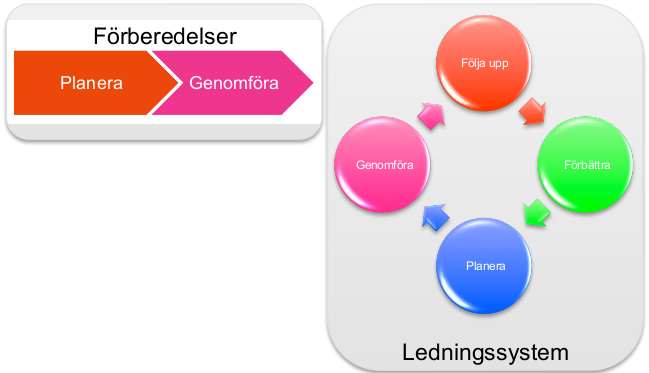
\includegraphics[height=0.5\textheight]{lis.png}
    \caption{Införande och genomförande av LIS.}
  \end{figure}
\end{frame}

\begin{frame}{Projektplan}
  \begin{itemize}
    \item Utgör projektets grund.
    \item Definierar omfattningen och gränserna för LIS\@.
    \item Ett avtal som är bra för både projektledare och ledning.
    \item Kan innehålla:
      \begin{itemize}
        \item Bakgrund och behov,
        \item syftet med projektet,
        \item mål,
        \item omfattning och avgränsning,
        \item kopplingar och kontaktytor,
        \item tidsplan, och
        \item budget.
      \end{itemize}
  \end{itemize}
\end{frame}

\begin{frame}{Projektorganisation}
  \begin{itemize}
    \item Viktigt med bredd: att representera hela organisationen.
    \item Viktigt med rätt kompetens: projektledning och informationssäkerhet.
    \item Viktigt med mandat!
    \item Organisationen bör vara aktiv och engagerad för att inte kompetensen 
      ska försvinna efter projektets slut.
  \end{itemize}
\end{frame}

\begin{frame}{En kort checklista}
  \begin{itemize}
    \item Har ledningen fattat beslut om att arbeta för att implementera LIS\@?
    \item Har ledningen utsett någon som samordnar organisationens 
      informationssäkerhet?
    \item Har ledningen sett till att det finns en strategi för att kommunicera 
      LIS-arbetet internt?
    \item Har ledningen fattat beslut gällande resurser?
  \end{itemize}
\end{frame}


\section{Analysera}

\subsection{Verksamhetsanalys}

\begin{frame}{Vad ska skyddas?}
  \begin{itemize}
    \item Vilka informationstillgångar har vi och hur skyddsvärda är de?
    \item Vad menas med att skydda dem?
  \end{itemize}
\end{frame}

\begin{frame}{Verksamhetsanalys}
  \begin{itemize}
    \item Verksamhetsanalysen syftar till att identifiera 
      informationstillgångar, samt

    \item hur skyddsvärda de är.

    \item Ska leda till en strukturerad förteckning över
      \begin{itemize}
        \item vilka informationstillgångar som finns,
        \item vilka krav och förväntningar som finns på dessa, samt
        \item vilket värde respektive tillgång har.
      \end{itemize}

  \end{itemize}
\end{frame}

\begin{frame}{Exempel på informationstillgångar}
  \begin{itemize}
    \item Medarbetare: kvalifikationer, erfarenheter.
    \item Data: databaser, avtal, dokumentation, prover, rutiner.
    \item Programvarutillgångar: tillämpningsprogram, systemprogram, 
      utvecklingsprogram.
    \item Tjänster: data- och kommunikationssystem, försörjningssystem.
    \item Immateriella: rykte, profil.
    \item Fysiska: datorutrustning, flyttbar datamedia.
  \end{itemize}
\end{frame}

\begin{frame}{Uppdelning av informationstillgångar}
  \begin{description}
    \item[Primära] Avser den huvudsakliga informationen; exempelvis ritning, 
      logg och avtal.

    \item[Sekundära] Avser resurser som krävs för att hantera de primära 
      informationstillgångarna.

  \end{description}
  Vad händer när du inte längre har kvar programmet som kan läsa det 
  proprietära slutna formatet som informationen finns lagrad i?
\end{frame}

\begin{frame}{Hitta informationstillgångarna}
  \begin{itemize}
    \item Tidigare kartläggningar?
    \item Avdelningsvis?
    \item IT-system?
    \item Projekt?
    \item Processer?
    \item Funktionsvis?
  \end{itemize}
\end{frame}

\begin{frame}{Krav på informationstillgångarna}
  \begin{itemize}
    \item För att kunna klassificera behövs kraven kännas till.

    \item Behöver objektivt sätt att mäta vikten av skydd.
      \begin{itemize}
        \item Min information är viktigast!
      \end{itemize}

    \item Vilken information är viktig för att verksamheten ska gå att bedriva?

  \end{itemize}
\end{frame}

\begin{frame}{Legala krav}
  Avtal lagar och förordningar.
  \begin{itemize}
    \item PUL,
    \item Arkivlagen,
    \item Offentlighets- och sekretesslagen,
    \item MSBFS 2009:10,
    \item Säkerhetsskyddslagen.
  \end{itemize}
\end{frame}

\begin{frame}{Interna krav}
  Krav som verksamheten ställer upp för att nå sina mål.
  Exempelvis:
  \begin{itemize}
    \item Vision,
    \item affärsidé,
    \item policyer,
    \item värdegrund.
  \end{itemize}
\end{frame}

\begin{frame}{Informationsklassificering}
  \begin{itemize}
    \item Metod för att värdera hur skyddsvärd en informationstillgång är.

    \item För att kunna skapa ett lämpligt skydd.

    \item Värderar respektive tillgång utifrån:
      \begin{itemize}
        \item tillgänglighet,
        \item riktighet,
        \item konfidentialitet.
      \end{itemize}

    \item Varje perspektiv har ett antal skyddsklasser.

  \end{itemize}
\end{frame}

\begin{frame}{MSB:s förslag på klassificeringsmodell}
  \begin{figure}
    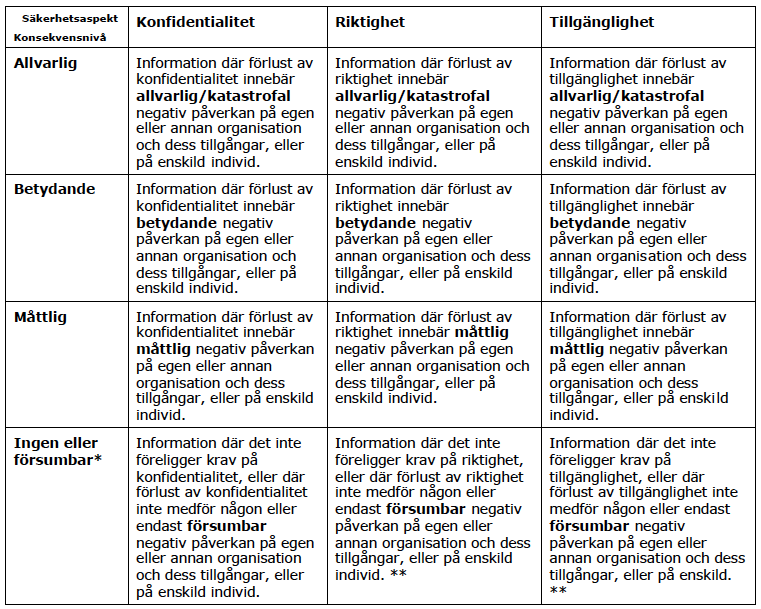
\includegraphics[height=0.7\textheight]{msb-klassificering.png}
    \caption{MSB:s förslag på klassificeringsmodell.}
  \end{figure}
\end{frame}

\begin{frame}{Informationsklassificering}
  \begin{itemize}
    \item Alla tillgångar klassificeras mot alla identifierade krav ur alla 
      perspektiv.
    \item Informationsägaren klassificerar.
    \item Anpassa gärna modellen efter verksamheten.
  \end{itemize}
\end{frame}

\begin{frame}{Universitetets förslag på klassificeringsmodell}
  \begin{figure}
    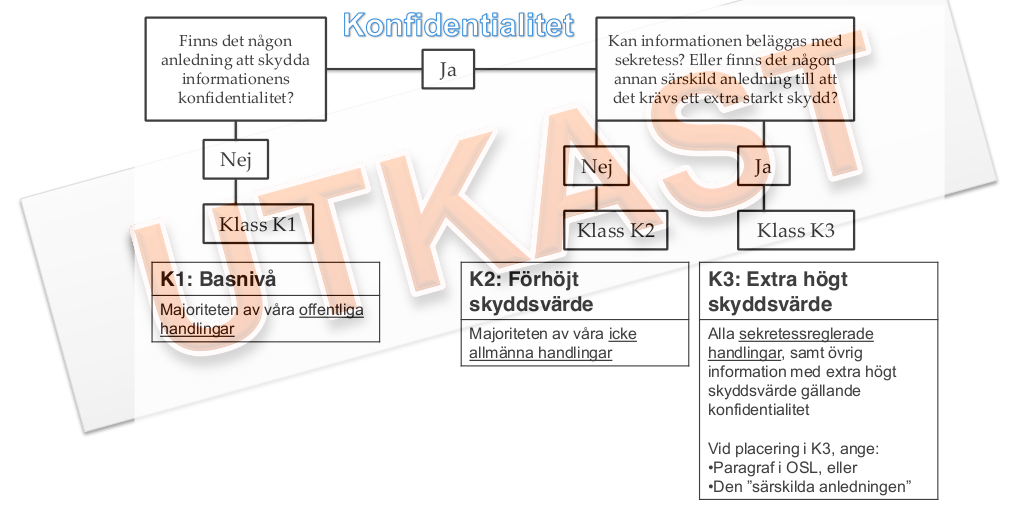
\includegraphics[width=\textwidth]{miun-klassificering.png}
    \caption{Universitetets förslag på klassificeringsmodell för 
    konfidentialitet.}
  \end{figure}
\end{frame}

\begin{frame}{Universitetets förslag på klassificeringsmodell}
  \begin{figure}
    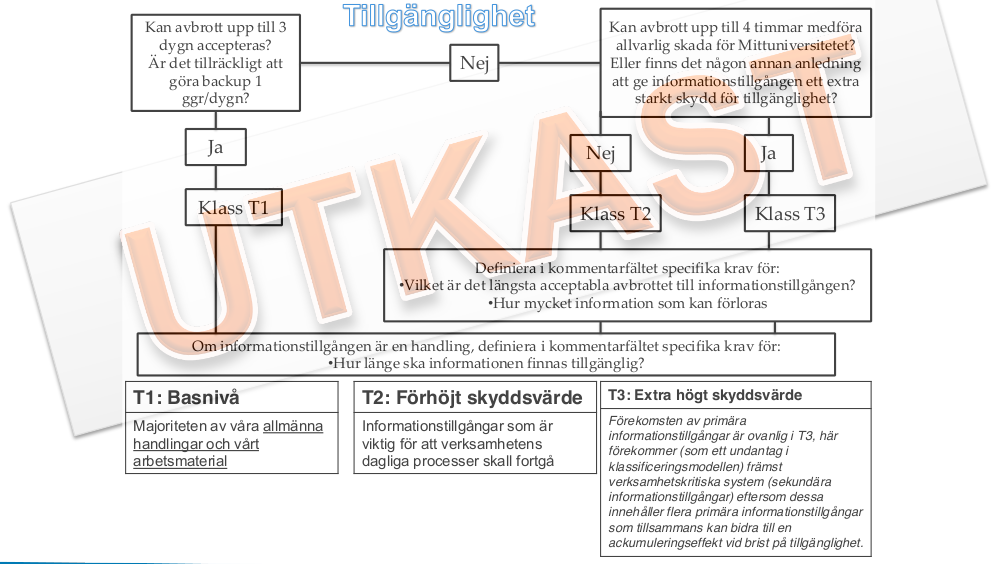
\includegraphics[width=\textwidth]{miun-tillganglighet.png}
    \caption{Universitetets förslag på klassificeringsmodell för 
    tillgänglighet.}
  \end{figure}
\end{frame}

\begin{frame}{Universitetets förslag på klassificeringsmodell}
  \begin{figure}
    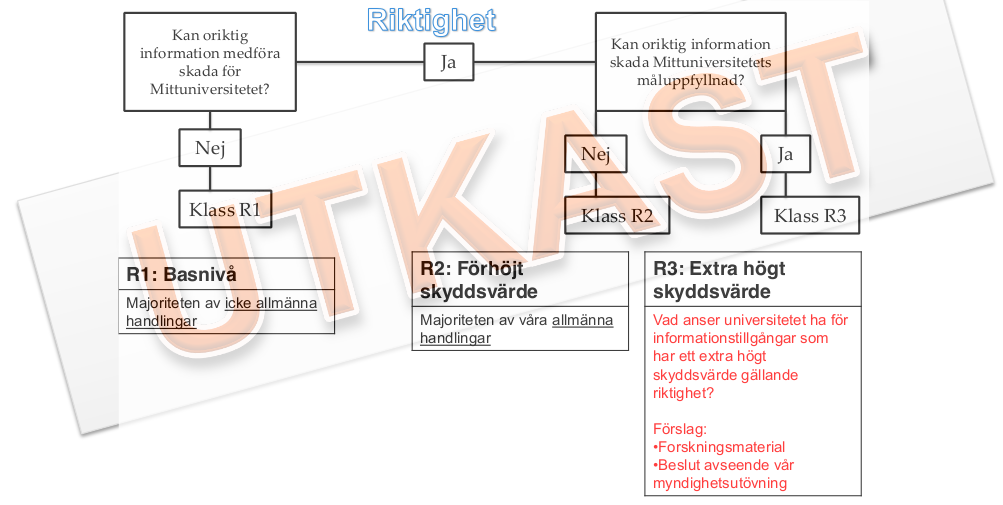
\includegraphics[width=\textwidth]{miun-riktighet.png}
    \caption{Universitetets förslag på klassificeringsmodell för riktighet.}
  \end{figure}
\end{frame}

\begin{frame}{Exempel på resultat från universitetet}
  \begin{figure}
    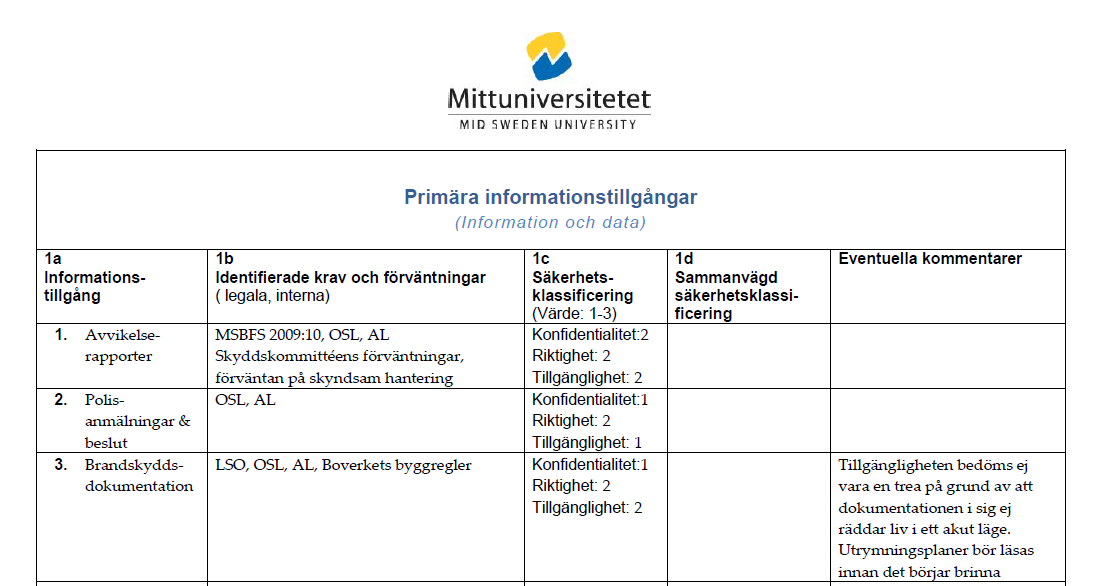
\includegraphics[width=\textwidth]{miun-klassresultat.png}
    \caption{Del av universitetets resultat.}
  \end{figure}
\end{frame}

\subsection{Riskanalys}

\begin{frame}{Riskanalys}
  Måste göra avgränsningar:
  \begin{itemize}
    \item Vilka informationstillgångar vill man göra riskanalys på?
    \item Vilka tillgångar är inte tillräckligt kritiska för en riskanalys?
  \end{itemize}
\end{frame}

\begin{frame}{Riskanalys}
  \begin{itemize}
    \item Används för att anpassa skyddet efter verksamhetens tillgångar.
    \item Genererar en förteckning över
      \begin{itemize}
        \item befintliga hot,
        \item hotens skadeverkningar, och
        \item förslag på riskhantering.
      \end{itemize}
  \end{itemize}
\end{frame}

\begin{frame}{Identifiera hot}
  \begin{itemize}
    \item Använd brainstorming för att ta fram förslag på hot.
    \item Ta med alla förslag!
    \item Var specifik: avsiktligt eller oavsiktligt informationsläckage.
    \item Exempel:
      \begin{itemize}
        \item Medarbetare avsiktligt saboterar ett system.
        \item Medarbetare snubblar i nätverkskablarna som är dragna på golvet.
        \item Buggar i programvara.
        \item Brand, översvämning.
      \end{itemize}
  \end{itemize}
\end{frame}

\begin{frame}{Riskmatris}
  \begin{figure}
    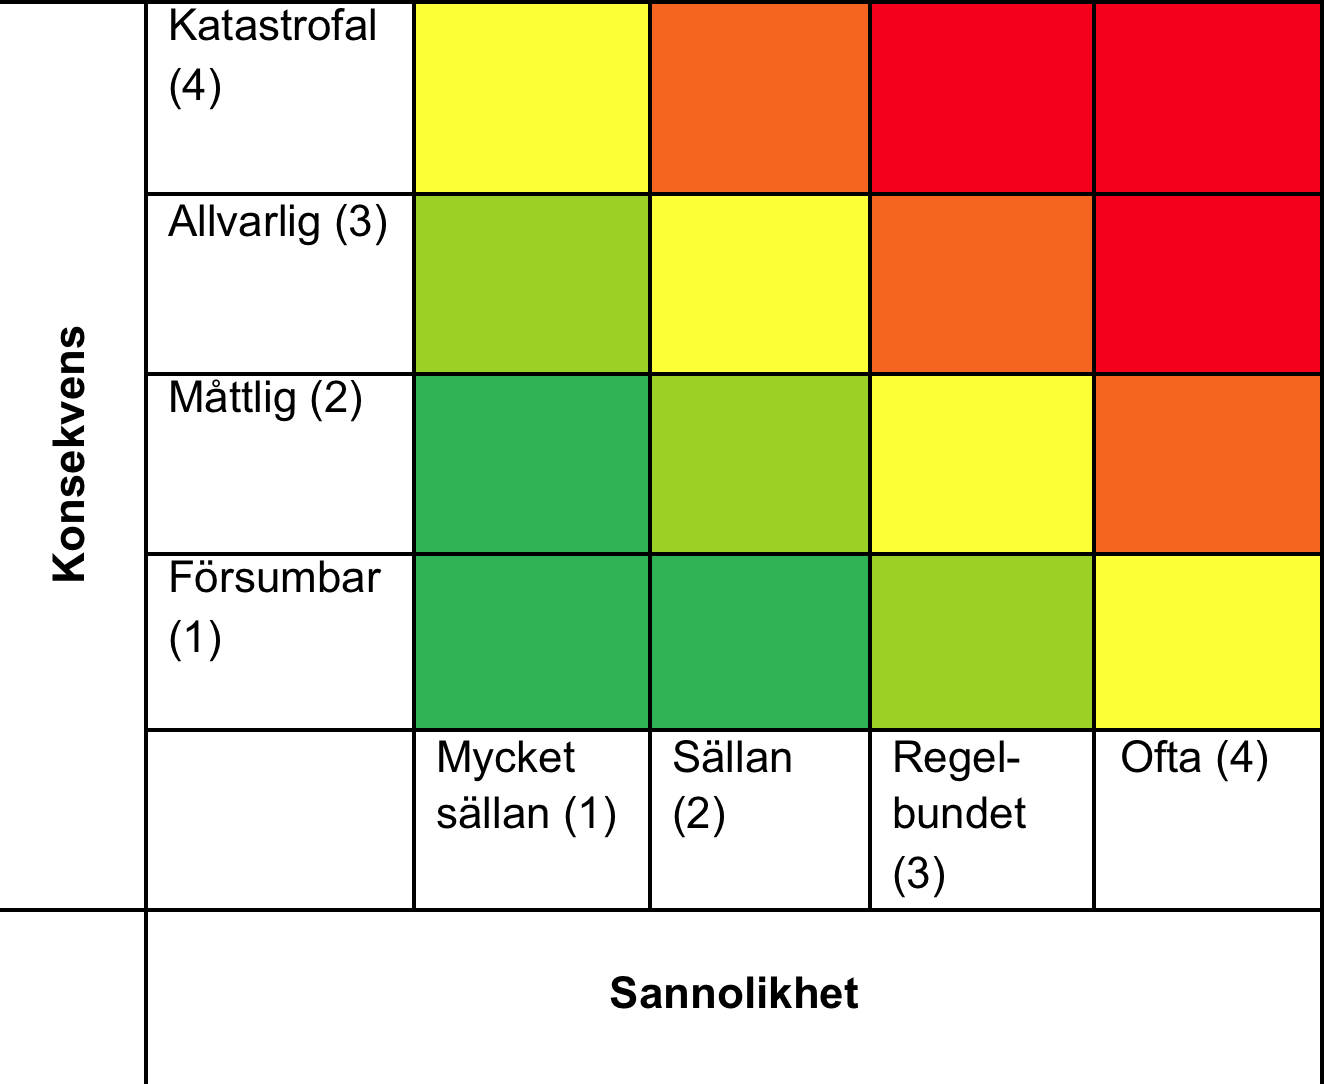
\includegraphics[height=0.7\textheight]{riskmatris.png}
    \caption{En riskmatris.}
  \end{figure}
\end{frame}

\begin{frame}{Riskmatris}
  \begin{itemize}
    \item Bedöm sannolikhet och konsekvens av varje enskilt hot och placera dem 
      i matrisen.
    \item Fokus för konsekvenser är konsekvenser för verksamheten.
    \item Ger visualiserat resultat, lättöverskådlig grund för prioritering av 
      säkerhetsåtgärder.
  \end{itemize}
\end{frame}

\begin{frame}{Riskmatris}{Konsekvenser}
  \begin{itemize}
    \item Hur allvarlig blir konsekvensen för verksamheten om hotet blir 
      verklighet?
    \item Klargör för \emph{vem} det blir en konsekvens: verksamheten genom 
      bieffekt av konsekvenser för samhället?
    \item Underlättar att ange exempel för de olika nivåerna, exempelvis: 
      kostnader, försämrat rykte, \dots
  \end{itemize}
  \begin{center}
    Allvarlig -- Betydande -- Måttlig -- Försumbar
  \end{center}
\end{frame}

\begin{frame}{Riskmatris}{Sannolikhet}
  \begin{itemize}
    \item Hur troligt är det att hotet inträffar?
    \item Underlättar med exempel för nivåerna: år, veckor, dagar?
  \end{itemize}
  \begin{center}
    Mycket sällan -- Sällan -- Regelbundet -- Ofta
  \end{center}
\end{frame}

\begin{frame}{Riskbehandling}
  \begin{itemize}
    \item Besluta om de identifierade hoten ska åtgärdas eller accepteras:
      \begin{itemize}
        \item Acceptera,
        \item eliminera,
        \item överföra,
        \item behandla.
      \end{itemize}
    \item Vilka åtgärder ska vidtas?
  \end{itemize}
\end{frame}

\begin{frame}{Möjliga åtgärder}
  \begin{itemize}
    \item Administrativ säkerhet:
      \begin{itemize}
        \item Styrdokument,
        \item kunskapshöjande åtgärder.
      \end{itemize}
    \item Fysisk säkerhet:
      \begin{itemize}
        \item Tillträdeskontroll,
        \item låsta arkivskåp.
      \end{itemize}
    \item IT-säkerhet:
      \begin{itemize}
        \item Bradväggar,
        \item kryptering,
        \item fler under kursens gång.
      \end{itemize}
  \end{itemize}
\end{frame}

\begin{frame}{Exempel från universitetet}
  Hemligt forskningsmaterial med stort affärsintresse: K3, R2, T2.
  \begin{figure}
    \hfill
    \subfloat[Hotbild]{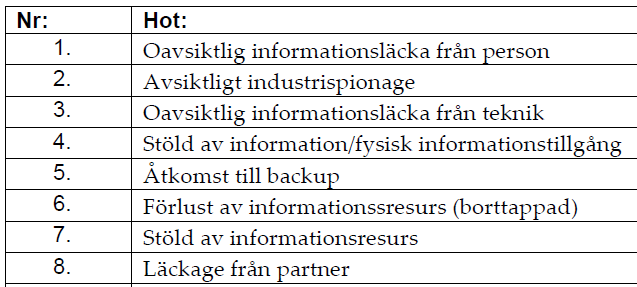
\includegraphics[width=0.4\textwidth]{miun-hot.png}}
    \hfill
    \subfloat[Risker]{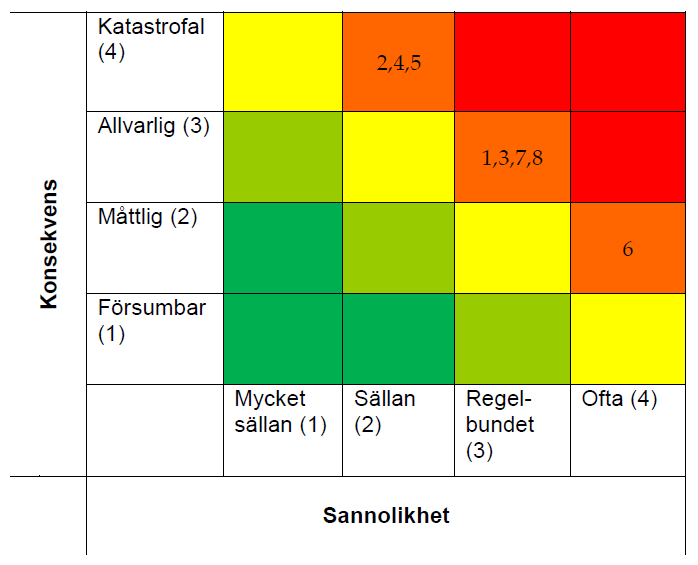
\includegraphics[width=0.4\textwidth]{miun-riskmatris.png}}
    \hfill
    \caption{Hotbild och bedömd risk.}
  \end{figure}
\end{frame}

\begin{frame}{Exempel från universitetet}
  \begin{figure}
    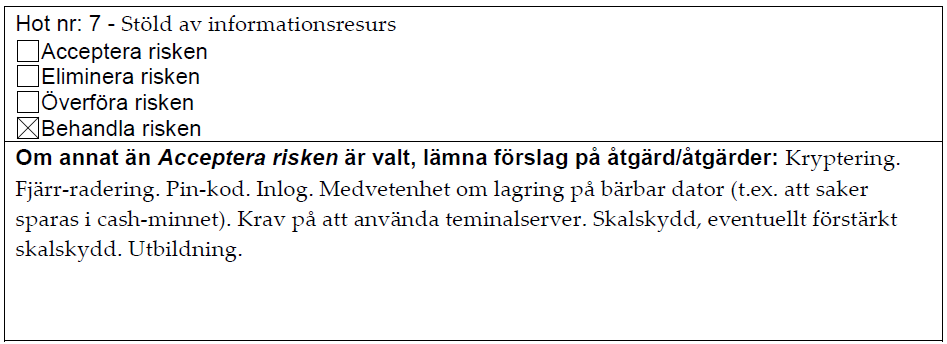
\includegraphics[width=\textwidth]{miun-atgard.png}
    \caption{Åtgärder för att bemöta hotet.}
  \end{figure}
\end{frame}

\begin{frame}{Slutligen---när ska analyserna göras?}
  \begin{itemize}
    \item Årligen.
    \item Vid förändrad verksamhet.
    \item Vid planering av ny verksamhet.
  \end{itemize}
\end{frame}


\section[Uppgifter]{Examinationsuppgifter}

\begin{frame}{Examinationsuppgifter}
  \begin{itemize}
    \item M1 Ledningssystem för informationssäkerhet.
    \item M2 Verksamhets- och riskanalys.
    \item S3 Verksamhets- och riskanalys.
  \end{itemize}
\end{frame}


%%%%%%%%%%%%%%%%%%%%%%

\begin{frame}[allowframebreaks]{Referenser}
	\small
  \printbibliography{}
\end{frame}

\end{document}

